% CT-3: a protocol read as a morphism in a strict monoidal category — role wires, with
% interactions as boxes. The monoidal tensor ⊗ partitions roles into independent factors;
% roles in different factors PROVABLY never communicate (the Mixture pattern). Palette:
% orchestrator wire=indigo, specialist factors=sky, interaction box=emerald.
\documentclass[border=10pt]{standalone}
\usepackage{tikz}
\usepackage{amsmath}
\usepackage{xcolor}
\usetikzlibrary{positioning, fit, backgrounds}
\definecolor{orch}{HTML}{4F46E5}
\definecolor{sp}{HTML}{0284C7}
\definecolor{act}{HTML}{059669}
\definecolor{ink}{HTML}{1E293B}
\definecolor{slate}{HTML}{475569}
\begin{document}
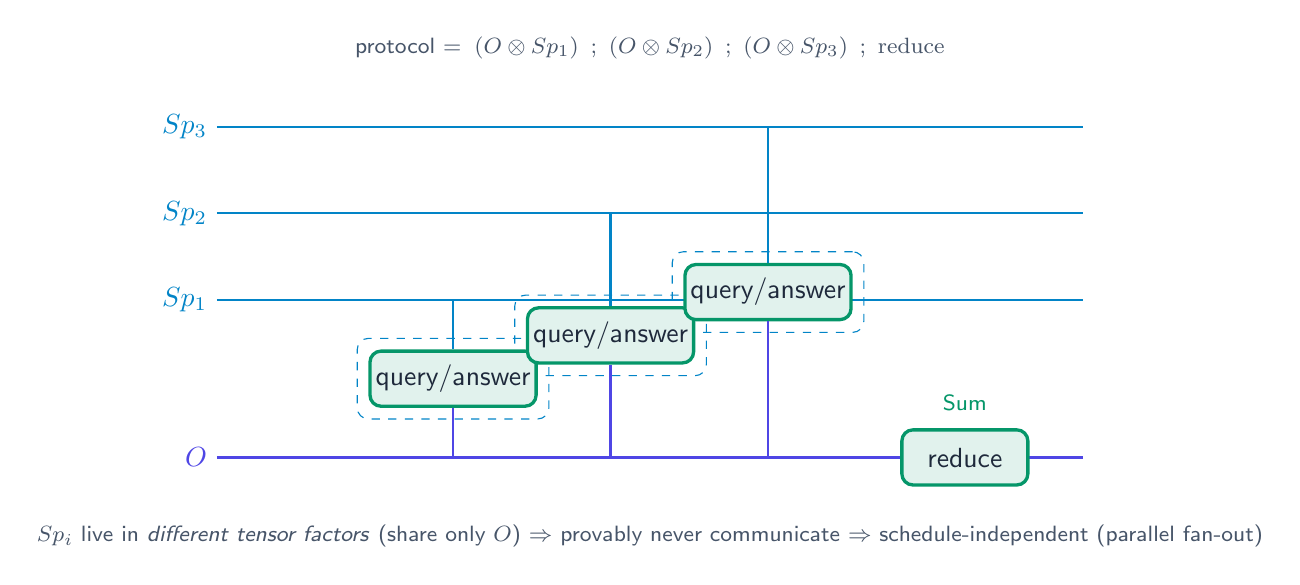
\begin{tikzpicture}[font=\sffamily,
    box/.style={draw=act, very thick, fill=act!12, rounded corners, minimum width=16mm, minimum height=7mm, inner sep=2pt, text=ink},
    wire/.style={thick}]

  % Orchestrator wire (central, shared).
  \draw[wire, orch] (0,0) -- (11,0);
  \node[orch, left] at (0,0) {$O$};

  % Specialist wires (each its own tensor factor).
  \foreach \y/\name in {2/Sp_1, 3.1/Sp_2, 4.2/Sp_3} {
    \draw[wire, sp] (0,\y) -- (11,\y);
    \node[sp, left] at (0,\y) {$\name$};
  }

  % Interaction boxes (O ⟷ each specialist) — the only shared morphisms.
  \node[box] (b1) at (3,1) {query/answer};
  \node[box] (b2) at (5,1.55) {query/answer};
  \node[box] (b3) at (7,2.1) {query/answer};
  \draw[wire, orch] (3,0) -- (b1); \draw[wire, sp] (3,2) -- (b1);
  \draw[wire, orch] (5,0) -- (b2); \draw[wire, sp] (5,3.1) -- (b2);
  \draw[wire, orch] (7,0) -- (b3); \draw[wire, sp] (7,4.2) -- (b3);

  % Summarizer reduce.
  \node[box] (sum) at (9.5,0) {reduce};
  \node[act, above=1mm of sum, font=\sffamily\footnotesize] {Sum};

  % Tensor-factor brackets (the disjoint partition).
  \begin{scope}[on background layer]
    \node[draw=sp, dashed, rounded corners, fit=(b1), inner sep=4pt] {};
    \node[draw=sp, dashed, rounded corners, fit=(b2), inner sep=4pt] {};
    \node[draw=sp, dashed, rounded corners, fit=(b3), inner sep=4pt] {};
  \end{scope}

  \node[slate, font=\sffamily\footnotesize, align=center] at (5.5,5.2)
    {protocol $=\; (O \otimes Sp_1) \;\mathbin{;}\; (O \otimes Sp_2) \;\mathbin{;}\; (O \otimes Sp_3) \;\mathbin{;}\; \mathrm{reduce}$};
  \node[slate, font=\sffamily\footnotesize, align=center] at (5.5,-1)
    {$Sp_i$ live in \emph{different tensor factors} (share only $O$) $\Rightarrow$ provably never communicate $\Rightarrow$ schedule-independent (parallel fan-out)};
\end{tikzpicture}
\end{document}
